%%%%%%%%%%%%%%%%%%%%%%%%%%%%%%%%%%%%%%%%%%%%%%
\section{Beamline instrumentations}
\label{sec:beaminstruments}

The H4 beamline will be instrumented with a number of detectors to provide information about the beam profile, position, momentum, and particle identification. A number of proposals are being evaluated for NP02 and NP04. In this section, the detector options are presented. 

\subsection{Beam profile and particle tracking}
Operation of the beam line needs at least one beam  monitor, able to provide the beam profile in two dimensions at the end of the beamline.   The beam monitor can also be exploited for data analisys, provided that it delivers data on an event-by-event basis. Another monitor, located immediately downstream of the last bending magnet, is added in the layout  in order to determine the particle  direction and position and match it with the reconstructed track in the LAr active volume.
\subsubsection{Fiber tracker}
The CERN Beam Instrumentation (BI) group offers to produce beam monitors base on scintillating fbres, that  are a mix between scintillators and optical fibres, having a polystyrene core surrounded by a cladding. Fibres provide a light yield ~8000 photons/MeV deposited with fast rising and decay times: $\approx$1-3 ns. The base design foresees 1mm square fibres in two planes to provide X and Y coordinates, having a  mirror on one end to increase
light collection.  Every monitor having two planes of 1~mm fibres adds 0.47\% $X_0$ to the material budget.
192 fibres per plane with no space between them will ensure a  192mmx192mm covered area, fitting in the beamline.
Light can be read either with MultiAnode PMTs or with SiPMs, depending on the application (see below about the possible use for Time of Flight).
Theese monitors are designed to work inside the vacuum chamber, mounted on special flanges, with no need to break the vacuum.

\subsubsection{Multiwire Proportional Chambers}
Fermilab has multi-wire proportional chambers (MWPCs) with X-Y sense plane
readout, approximately 128 mm x 128 mm, readily available that can be used as or in addition to beam profile monitors. Chambers add 0.002 nuclear collision lengths and 0.007
radiation lengths. These chambers have a long history, so installation, integrationand commissioning should be straightforward. They are operated in air, tus would need sectioning of the beamline vacuum.

\subsection{Momentum measurements}
The uncertainty in momentum resolution of the beam can be reduced by measuring the momentum particle by particle with a set of three detectors placed one before and two after one of the bending magnets. On paper, momentum resolutions of the order of 1\% could be achieved with this system, however  multiple scattering can affect the measurement at low energies. Preliminary results in full simulation point to a resulution better than 2\%. 
The same devices used for beam monitoring can be used also for momentum measurement.

\subsection{Particle identification}
The H4 beamline is capable of delivering two types of beam: electron and hadron beams. While the electron beam is relatively pure, the hadron beam consists of a mixture of electron, pion, kaon, and proton. Therefore it is essential to have efficient particle identification system to cleanly tag particle types on a particle by particle basis. To achieve this goal, a particle identification system based on a combination of threshold Cherenkov counters and Time-of-flight system are being considered for ProtoDUNEs. Cherenkov counters can be placed in the last segment of the beam line, in between the last bending magnet and the cryostat. Space for a ToF system is available provided that the detectors are compact enough, ensuring a flight path of about 23~m.

\subsubsection{Threshold Cherenkov counter}
The threshold Cherenkov counters have been used extensively in beamline to discriminate particles. Figure~\ref{fig:ckv} shows one of the counters used in the CERN test beam area. It consists of a gas radiator that is contained in a long cylindrical tube, and a detection box in which the Cherenkov light is reflected by a 45$^\circ$ mirror and focused onto a photomultiplier tube. The diameter of the cylindrical tube is designed to allow the counter to pass through the standard CERN beam pipe of about 20cm. A variety of gasses (e.g. CO2, nitrogen, argon, Freon 12, air, etc.) are available at CERN to optimize particle identification. The CERN beam group plans to install one thereshold Cherenkov counter in the H4 beamline. A second counter may be added to the beamline if additional funding is available. Figure~\ref{fig:ckv_gases} shows the momentum threshold for the production of Cherenkov light for various particles as a fuction of particle momentum for Freon 12 and CO$_2$ gases.
\begin{cdrfigure}[CERN threshold Cherenkov counter]{ckv}{CERN threshold Cherenkov counter}
  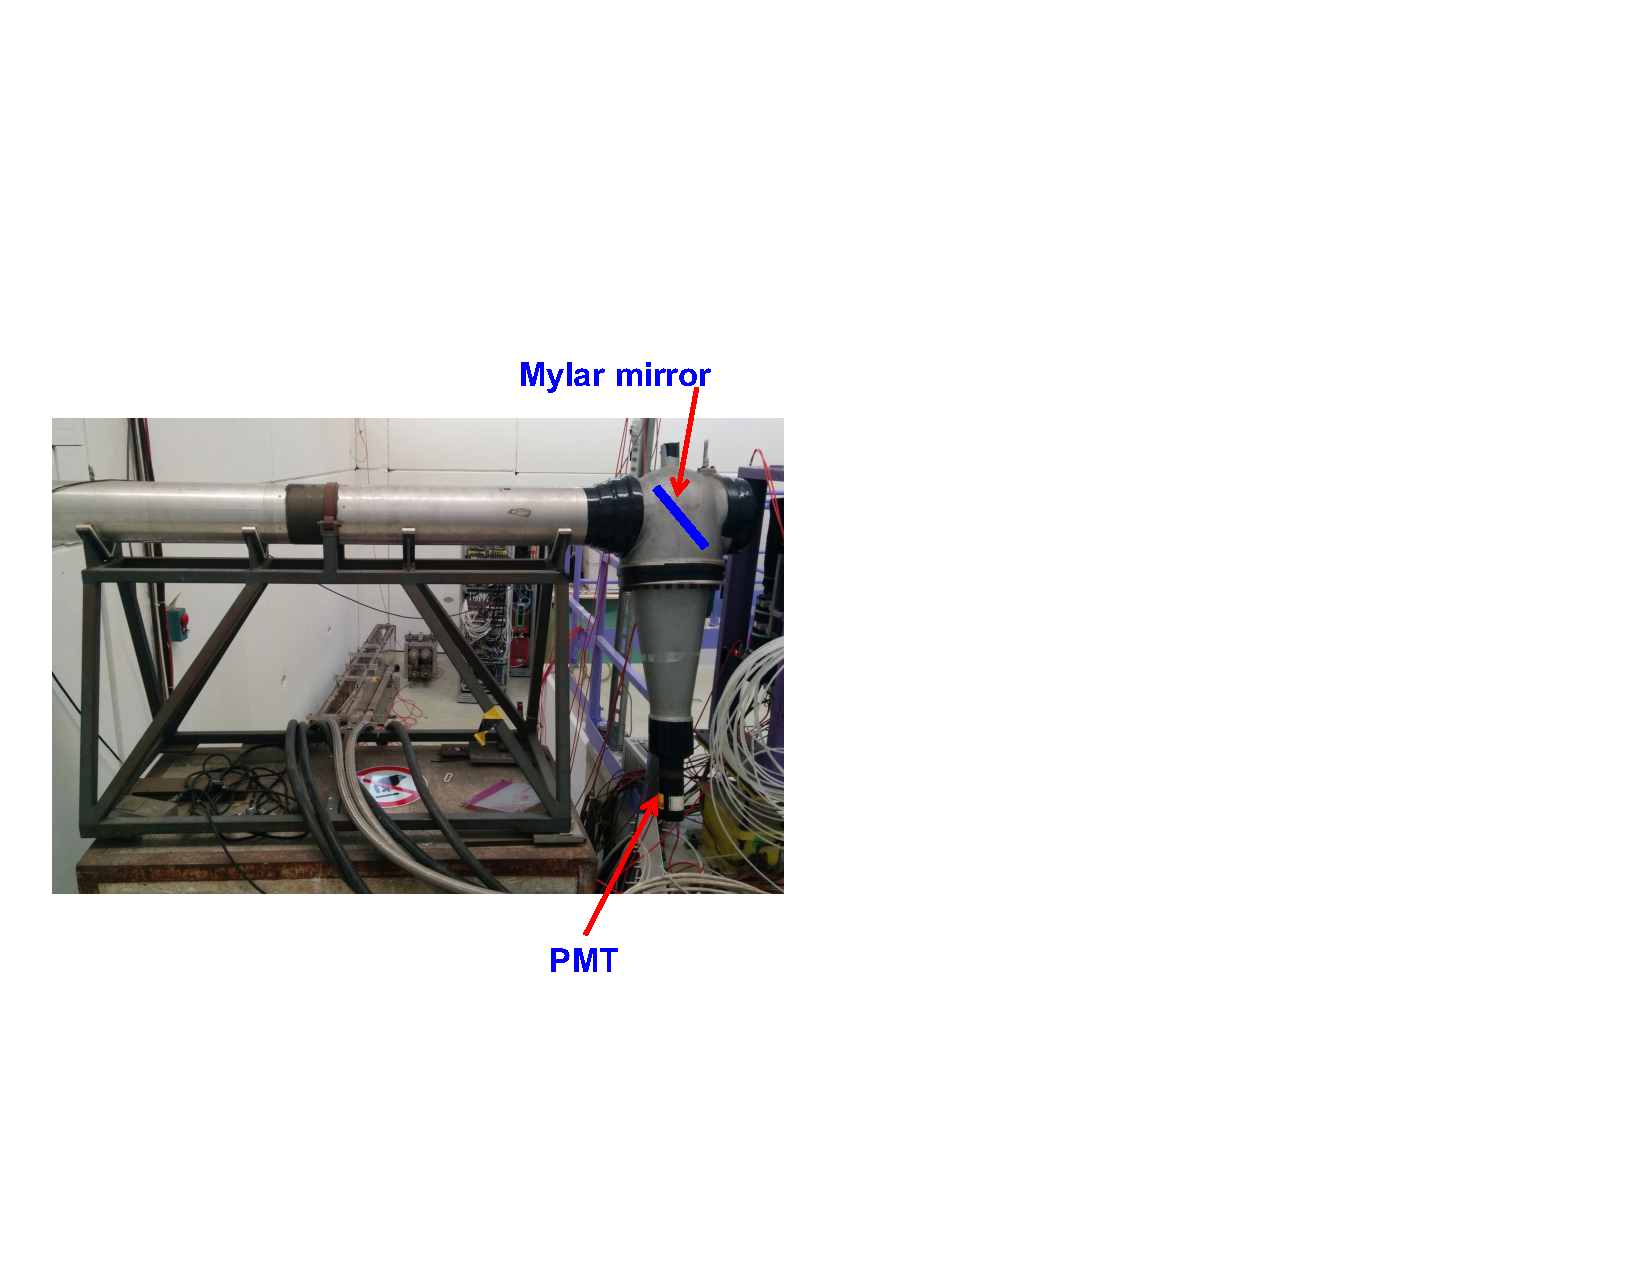
\includegraphics[width=0.65\textwidth]{beamline_ckv.pdf}
\end{cdrfigure}
\begin{cdrfigure}[Cherenkov gases]{ckv_gases}{Momentum threshold for the production of Cherenkov light for various particles as a function of particle momentum for Freon 12~\footnote{N. Charitonidis, Y. Karyotakis \it{et al.}, ``Hadron identification proposal for the ProtoDUNE experiments of CENF, to be published.} and CO$_2$ gases.}
  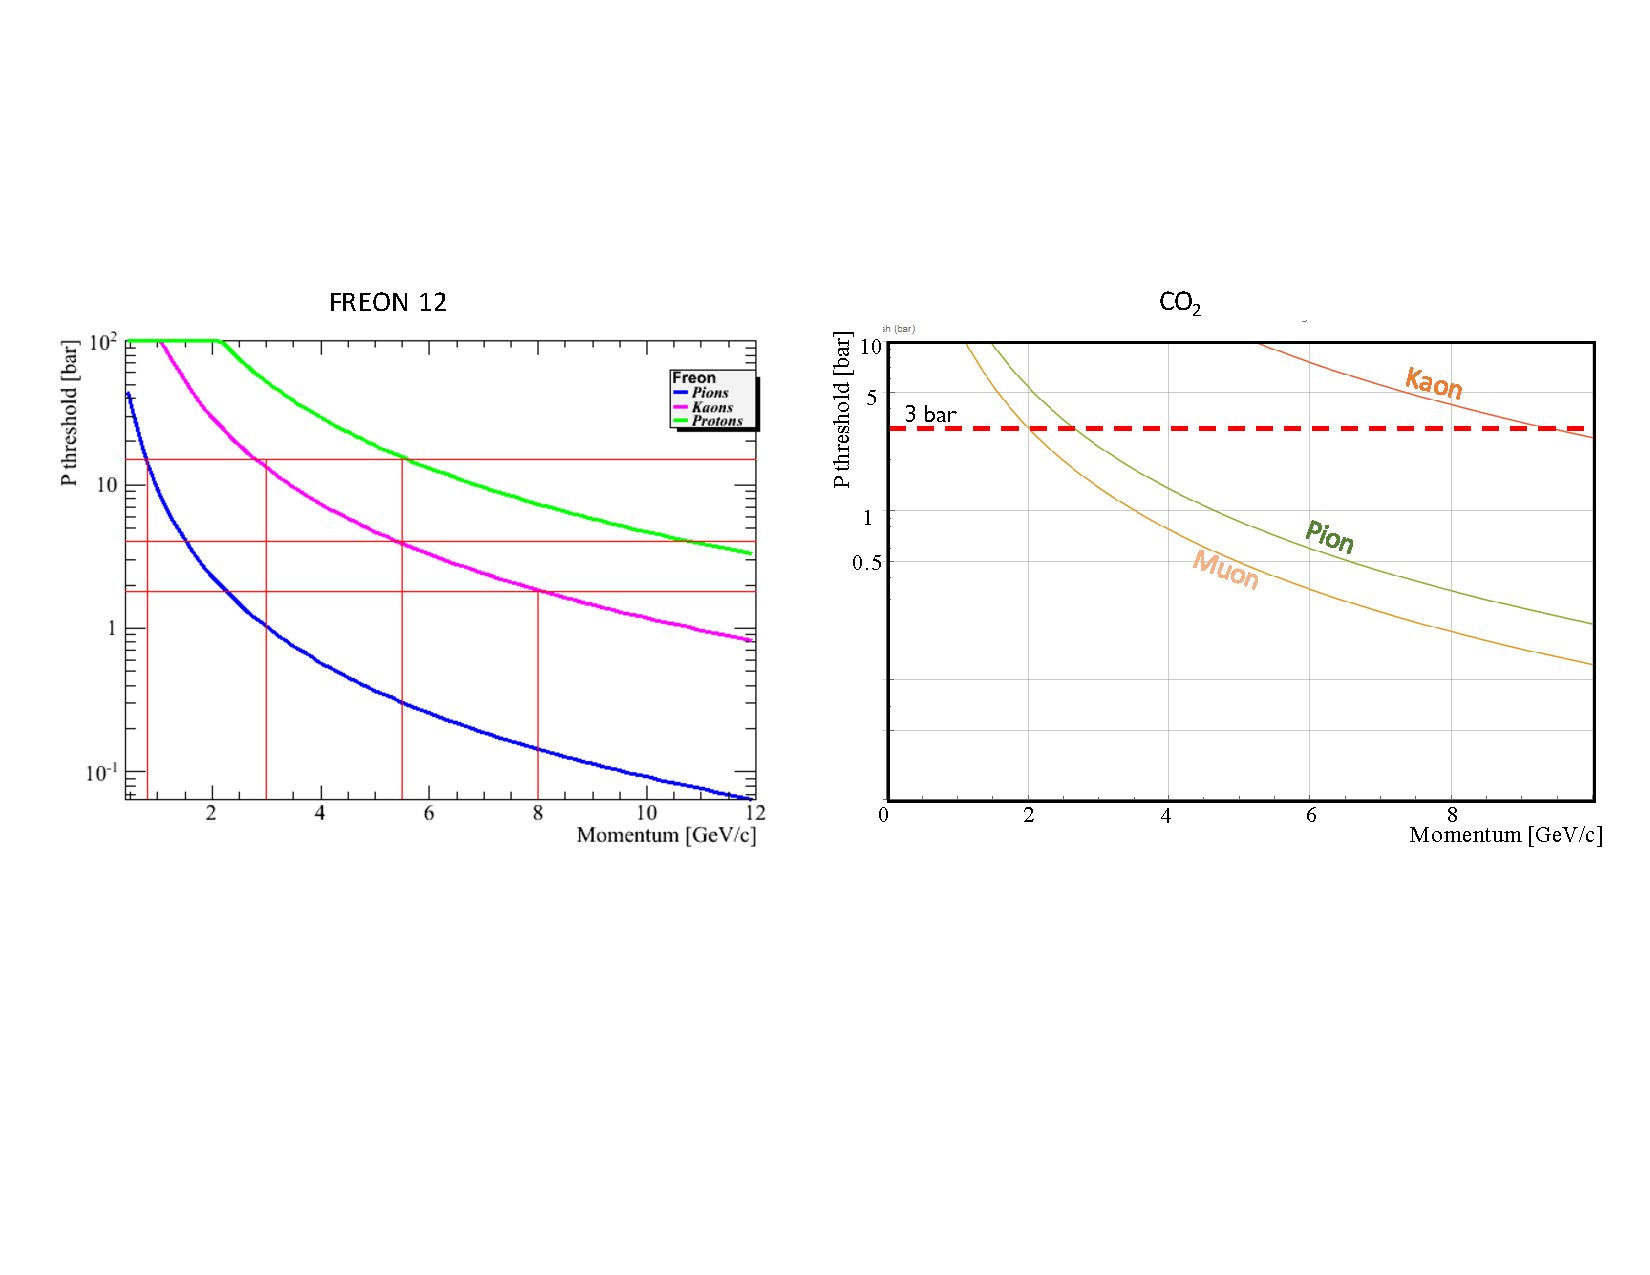
\includegraphics[width=0.99\textwidth]{beamline_CKVgases.pdf}
\end{cdrfigure}
Freon-12 has been selected for its high density, however it cannot be operated at pressures larger than 3bars to avoid liquefaction.  CO$_2$ can be pushed to higher pressures.  Drawings for high pressure Cerenkov counters exist at CERN, thus a new one could be manufactured. 
 Figure~\ref{fig:ckv_gases} shows that pions can be tagged with a 3bars Freon counter for momenta larger that 2 GeV/c, and Kaons can be tagged with an high pressure  CO$_2$  counter above 4 GeV/c. 
At low energies, it will be essential  to tag electrons, that are the dominant component of the beam. This can be easily achieved with one   of the cherenkovs filled with CO$_2$ at low pressure.

A time-of-flight system  is therefore needed to distinguish hadrons below the mentioned thresholds.  From table \ref{tab:beampartcomp} it is evident that the Kaon content of the beam is negligible at least below 2 GeV/c, thus  only pion-proton separation is needed at low energies. Figure\ref{fig:toftau} shows the ToF resolution needed to distinguish among particle species at $4\sigma$ as a function of the particle momentum, assuming a 23~m path. To distinguish pions from protons below 2 GeV/c a 1~ns resolution is enough, while ~300ps are necessary for kaon-proton up to  4~GeV/c. It has also to be noted that a ToF system with a ~100ps resolution would allow to identify protons from other hadrons up to 7~GeV, so that the high pressure CO$_2$ Cherenkov could be avoided. Conversely, in order to cover all the energy range up to ~7~GeV for all hadron  types, a ToF system with a resolution better than 40~ps would be needed.
In the following, two (possibly complementary) ToF systems are described.
\begin{cdrfigure}[Required ToF resolution]{toftau}{Required ToF resolution to  distinguish among particle species at $4\sigma$ as a function of the particle momentum, assuming a 23~m path }
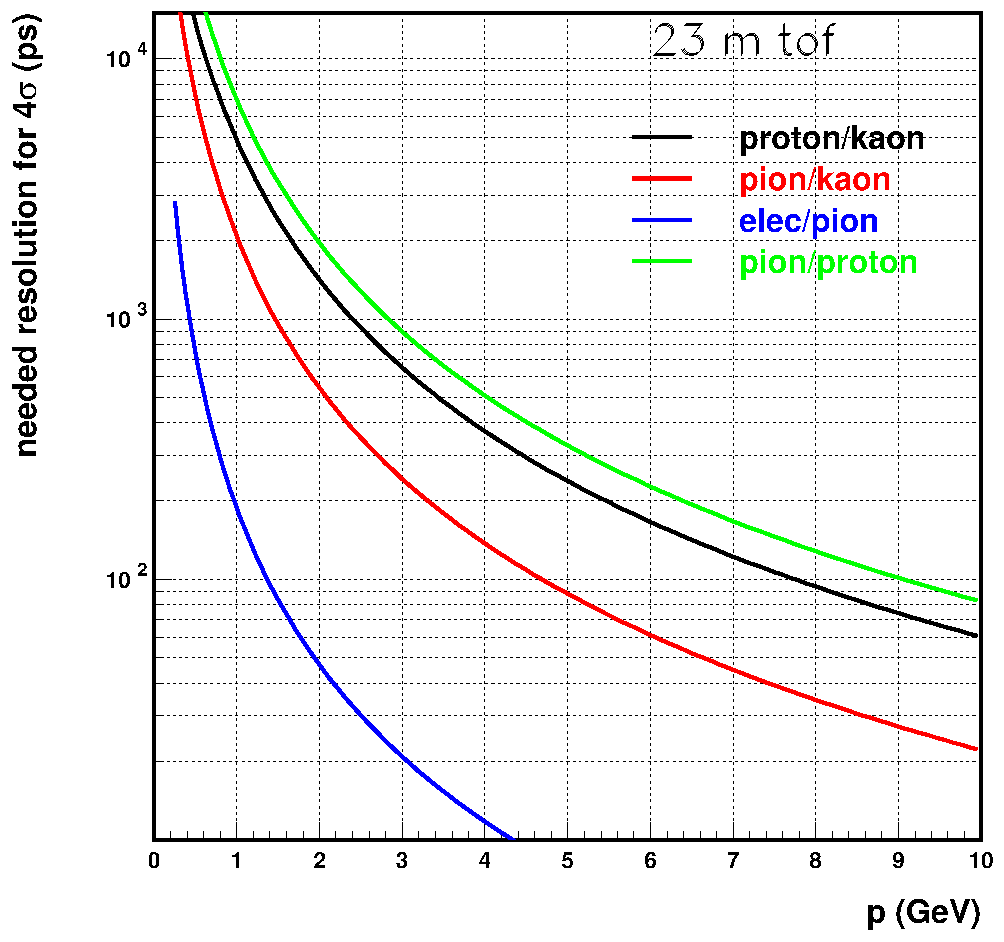
\includegraphics[width=0.95\textwidth]{toftaulow.pdf}
\end{cdrfigure}

\subsubsection{pLAPPD Time-of-flight system}
FermiLab is testing a ToF system that would utilize ANL 6 x 6 cm2
large-area picosecond photodetectors (pLAPPDs) (see figure \ref{fig:pLAPPD}).
 The MCP-based devices
are capable of $< 50$~ps resolution with gains of $10^6-10^7$,
mm-position resolution along one axis and slightly worse resolution
along the other axis.  The photodetector is mounted on a readout
board, so the relevant exterior dimensions are 165.1mm x 109.3mm and a
thickness of 16mm. The active area is defined by the 4 squares visible in figure \ref{fig:pLAPPD}, and amounts to about 8~cm$^2$.
\begin{cdrfigure}[pLAPPD]{pLAPPD}{Photo of one pLAPPD device as proposed for the H2 and H4 beamlines}
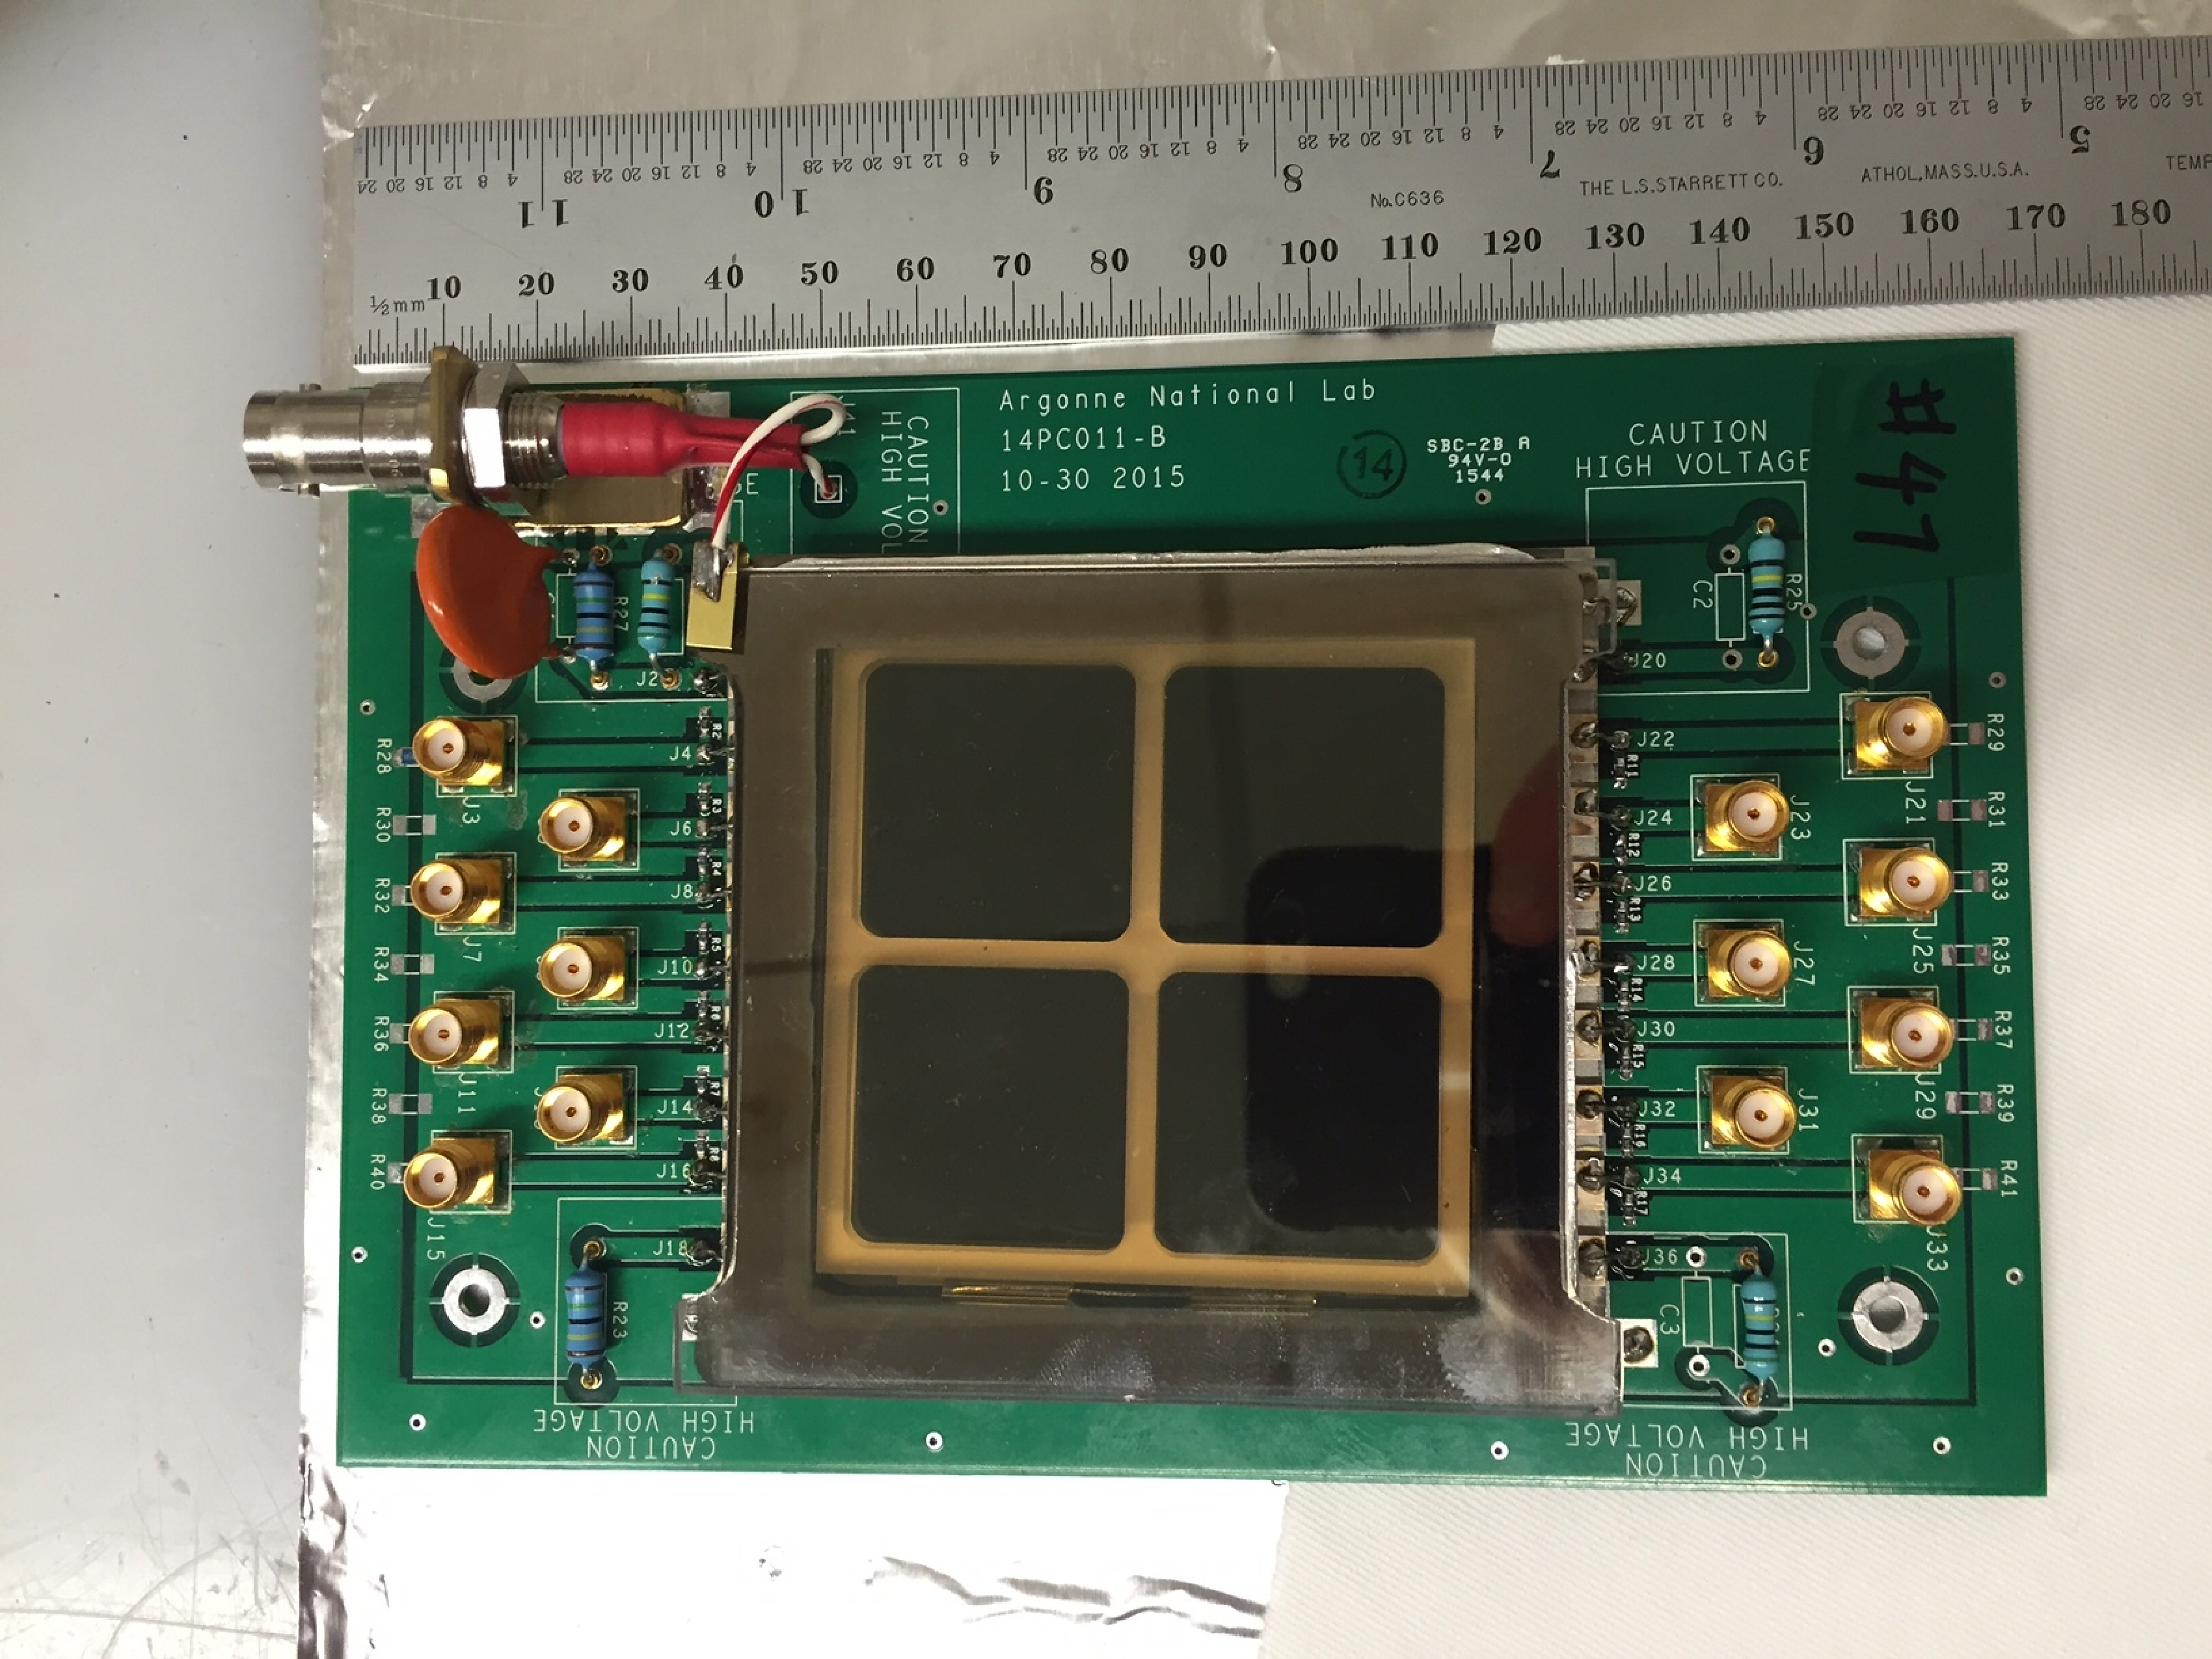
\includegraphics[width=0.95\textwidth]{LAPPD.pdf}
\end{cdrfigure}

\subsubsection{Other Time-of-flight system}
Investigation is ongoing on the possibility  to use the  scintillating fibres monitors for ToF purposes, aiming to a $\approx $ 1~ns resolution. The idea is to readout the detectors with the STiC ASIC for SiPM readout, developed at the  Kirchhoff Institute for Physics in Heidelberg. In this configuration, the time resolution would be dominated by the fibre response. A small prototype will be built and tested.
\subsection{Material Budget and discussion}
Summing up all the required instrumentaton, the ``full'' beam line should include 5 beam monitors (2 for tracking and 3 for spectrometry), two ToF devices, two 2~m long Cerenkovs at high density or pressure. The material budget would be much to high for operation at low mmenta, and in general for operation with electron beams.  
A full FLUKA simulation of materials in the beamline and of the ProtoDUNE detector, including the beam window details, has been used to evaluate the effect of materials. Since the final layout of the beamline optics was delivered only recently, the simulations presented here assume a straigt line with an initially parallel beam, deflected only by scattering. Particles are assumeed to be ``lost'' when scattered outside of the beam pipe. Imlementation of the magnetic elements is underway.
 Figure~\ref{fig:matblfull} shows the evolution of the material budget with a full instrumentation, assuming pLAPPD for ToF. The total, including the beam window, would arrive to $0.6X_0$, 0.15 interaction lengths, and an energy loss for a mip particle of 28~MeV.
The largest contribution comes from Cerenkov detectors and from the  ToF system. Cerenkovs are useless for low energies (except a low-pressure one for electron discrimination) and can be easily removed from the beamline and substituted with a section of vacuum pipe.  
In a situation without cerenkovs, the pLAPPD devices plus monitors would still account for almost  $0.2X_0$. Besides energy degradation, scattering of low energy particles would  further degrade the pion and proton content of the beam.  Figure~\ref{1GeVtof} show examples of the beam degradation due to materials at 1~GeV/c: The rate of pions arriving at the detector is reduced by a factor 2.5, and the energy spread rises to 1.2\% of The rate of protons stopping in the detector is reduced by a factor 4, and the energy is spread by 2\% rms. This calculation is done in optimistic conditions, that is neglecting the efficiency loss due to the small active area of the pLAPPD devices.

A possible way out would be the use of scintillating fibres as ToF devices for the lowes energy beams ($< 2 GeV$).  The feasibility of a fully plug-and-play beamline, with detectors going in and out, including those that need vacuum segmentation, is under discussion. It has also to be noted that a good performance of the ( combined) ToF system could avoid the use of non-standard CerenkoV counters.
 \begin{cdrfigure}[Material budget]{matblfull}{Material budget in the beam line, as a function of the distance from the centre of the detector (in cm). The red line describes the amount of $X-0$, the black line the amount of interaction length, both read on the left axis. The bleck dotted line is the average energy lost by a mip particle, and is read on the right axis (in MeV). Vertical lines show the positions of the various equipments (in between the two blue lines are the 3 devices for spectrometry, ``bm'' is the last beam monitor, ``bw'' is the starting point of the beam window)}  
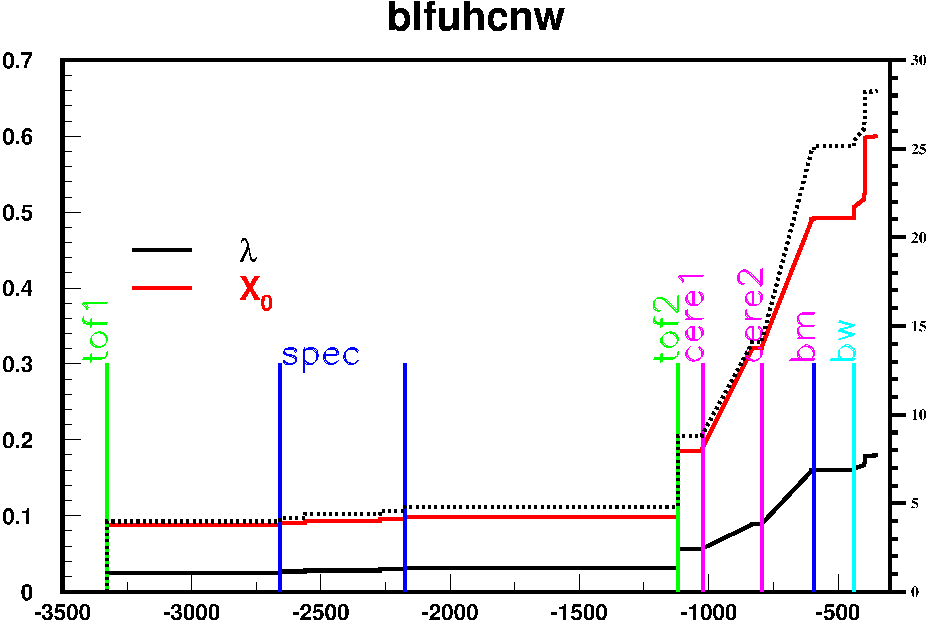
\includegraphics[width=0.95\textwidth]{blfuhcnwrayplo.pdf}
\end{cdrfigure}
 \begin{cdrfigure}[Effect of materials at  1GeV]{1GeVtof}{Effect of materials at  1GeV/c. Left: $\pi$ beam, energy of the particle entering in the detector, in three conditions: with  beam monitors, with beam monitors and pLAPPD for ToF, with the whole beamline filled with air (and no instrumentation). Right: proton beam, energy deposited by protons stopping in the LAr active volume, in three conditions: without instrumentation (the beam window is always present), with the scintillators only, and with scintillators plus pLAPPD for ToF.  }
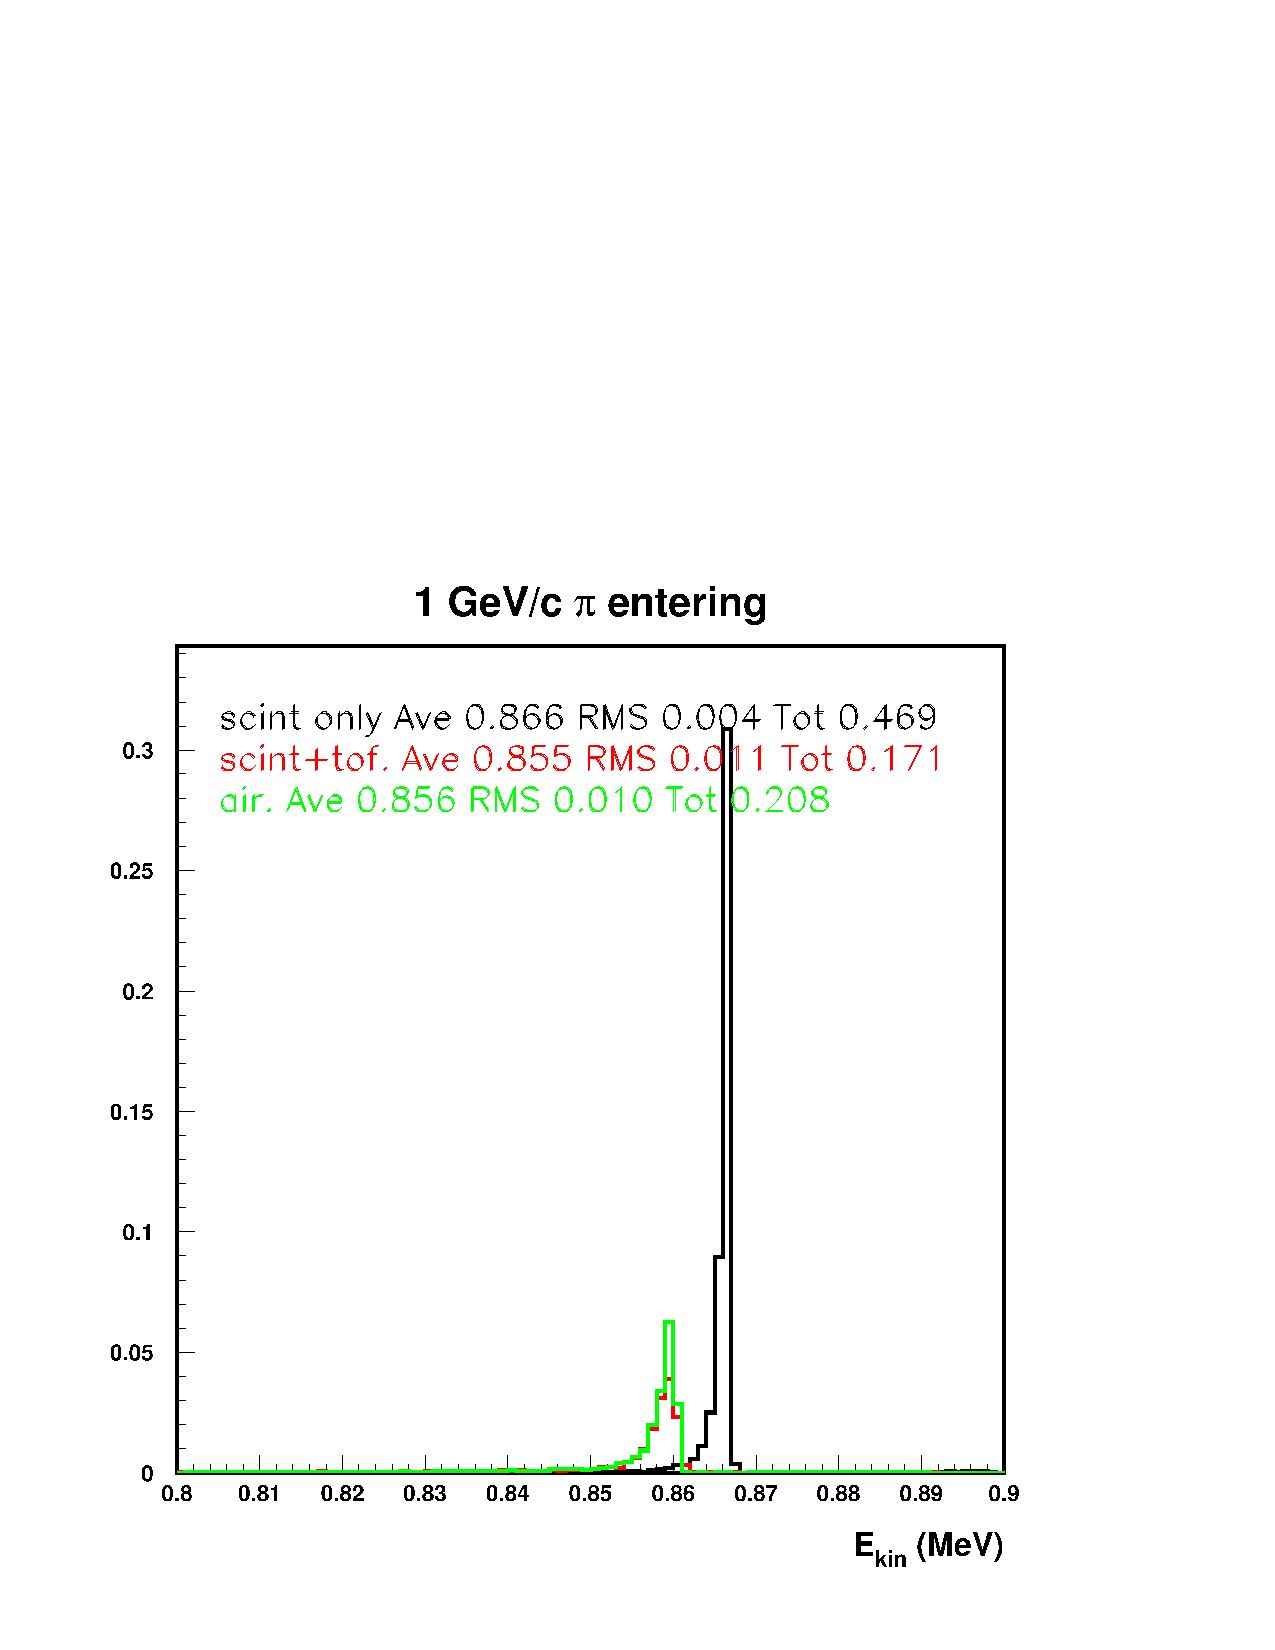
\includegraphics[width=0.48\textwidth]{pi1p0gev_innw.pdf}
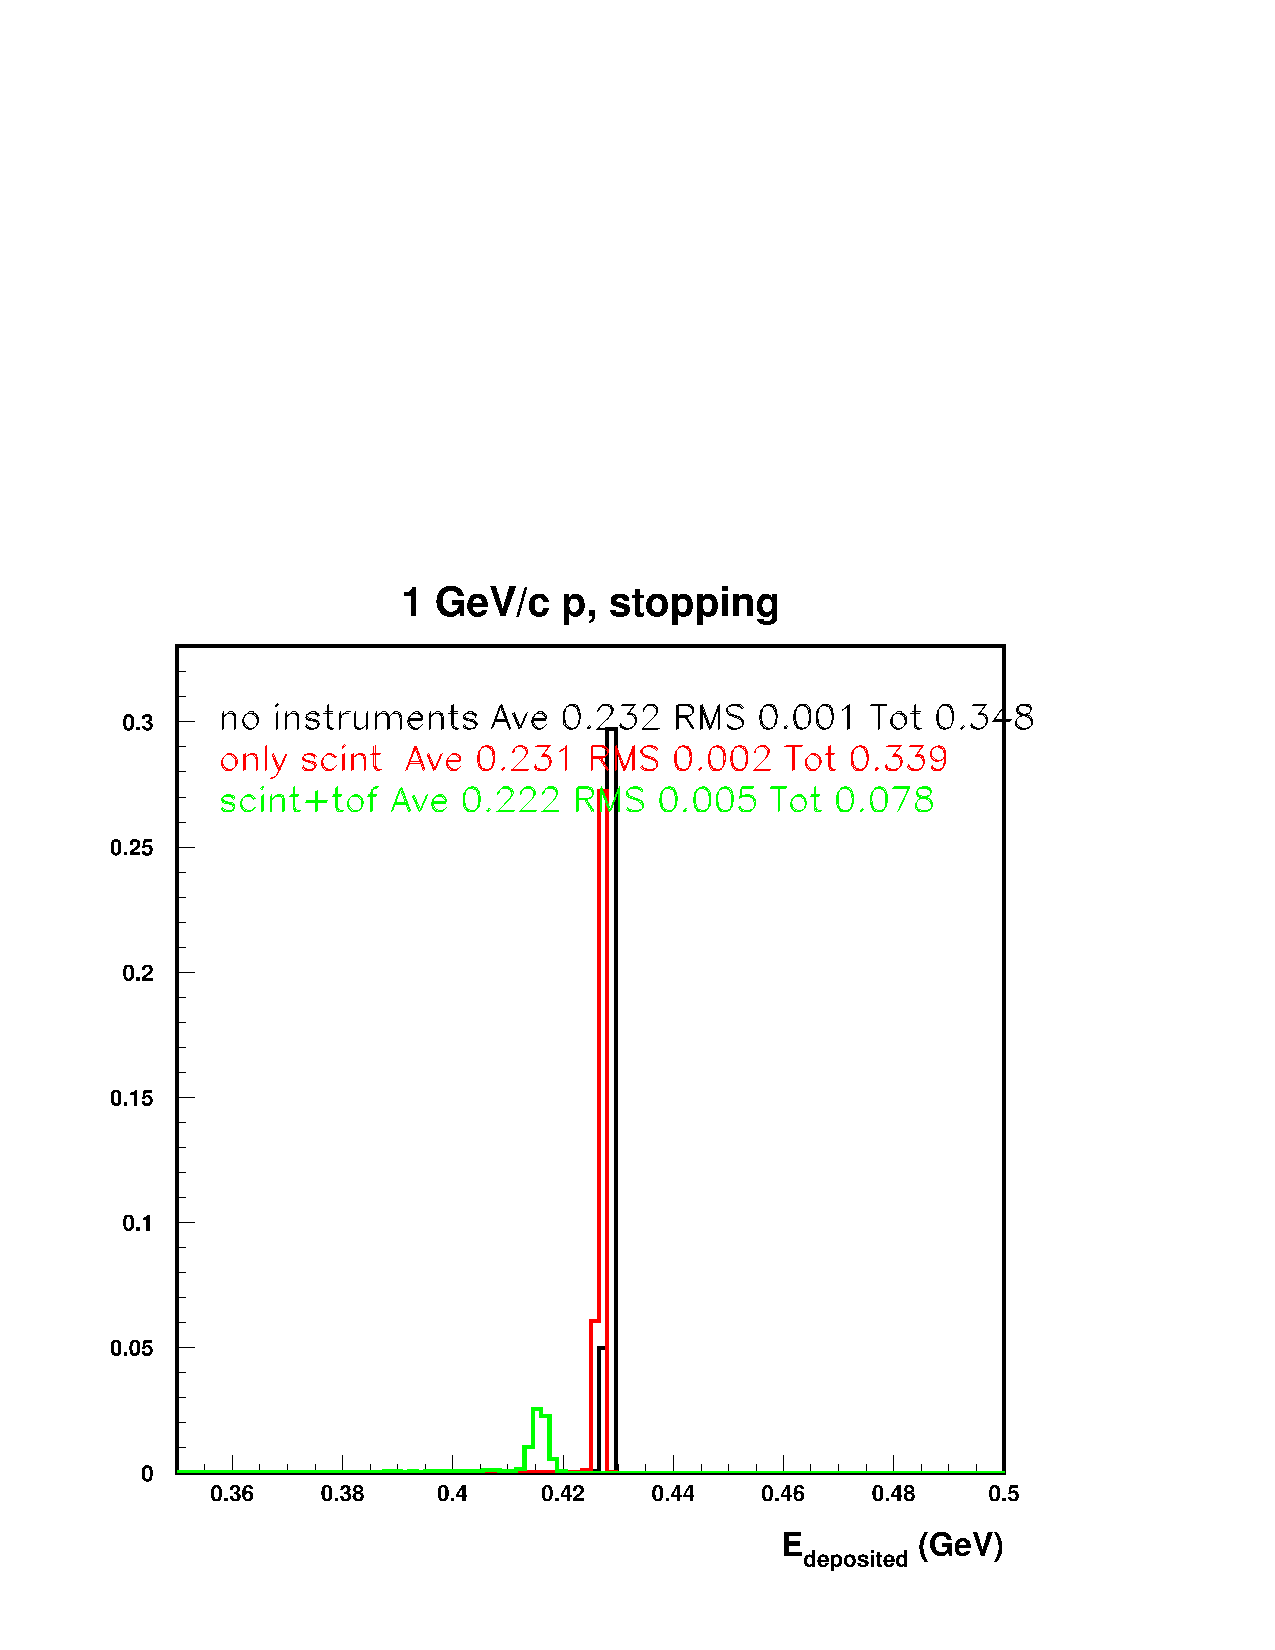
\includegraphics[width=0.48\textwidth]{p1gevstopnoqnw.pdf}
\end{cdrfigure}
  

\subsection {Trigger and data Acquisition}
Discussions are ongoing on how to provide a trigger signal from the beam instrumentation, and how to merge the beam instrumentation data into the TPC event. Syncronization will be ensured by a common time stamp through a White Rabbit network. White Rabbit is a fully deterministic Ethernet-based network for general purpose data transfer and synchronization. It can synchronize over 1000 nodes with sub-ns accuracy over fiber lengths of up to 10 km. It is developed and widely used at CERN.
